% Use class option [extendedabs] to prepare the 1-page extended abstract.
\documentclass[extendedabs]{bmvc2k}
\usepackage[colorlinks = true,
            linkcolor = blue,
            urlcolor  = blue,
            citecolor = blue,
            anchorcolor = blue]{hyperref}
\usepackage{kotex} % 한국어 사용 가능

% Document starts here
\begin{document}
\title{Style Transfer}
\addauthor{
Lee Gwan Hui$^1$, \today}{}{1}
\addinstitution{
$^1$2017142136, Department of Electrical and Electronic Engineering, Yonsei University.}
\maketitle
\let\thefootnote\relax\footnote{This is an extended abstract. The full paper is available at the \href{https://github.com/LeeGwanHui/TIL/tree/main/deeplearning_ham}{github}. }
\vspace{-0.2in}
\section{개요}
 \quad 다양한 deep learning task 중에서 이번 주차에서는 style transfer를 공부해볼 것이다.

 \section{Image Style Transfer Using Convolutional Neural Networks \cite{gatys2016image}}
 \subsection{motivation}
 \quad texture transfer라는 이름으로 한 이미지에서 다른 이미지로 style 정보를 넘기는 문제가 연구되고 있었다. 기존연구는 공통적으로 target의 low-level image features만으로 새로운 이미지를 만들어 낸다는 한계가 존재했다.
 style transfer의 경우에는 low-level feature이 아니라 target image의 high-level feature 즉 image에 존재하는 object의 일부분이나 혹은 전체 이미지를 포괄하는 feature 정보가 더 필요하다.
 따라서 CNN의 layer이 깊어질 수록 high level feature을 얻을 수 있다는 결과를 이용하여 high-level feature을 뽑고 이를 style transfer에 이용해보겠다는 것이다.
 이 논문은 최초로 CNN을 기반한 style transfer 모델이다.\cite{youtube_Style}
 
 \subsection{Method}
 \quad  network의 가중치를 고정한 뒤에 input image vector $\vec{x}$를 변환시키는 방법으로 새로운 이미지를 만든다. style transfer network의 특징 중 하나는 
input content 정보를 담은 이미지와 input style을 담은 이미지를 조합하여 새로운 이미지를 탄생시키는 것으로 각각의 loss를 구해서 이를 최소화 시켜주는 방법을 이 논문에서 사용했다.
따라서 loss function의 정의가 무엇보다 중요하다. 이 논문에서는 전체 loss를 아래와 같이 정의하였다.
$$L_{total}(\vec{p},\vec{a},\vec{x}) = \alpha L_{content}(\vec{p}, \vec{x} ) + \beta L_{style}(\vec{a},\vec{x})$$
위의 식에서 각각의 loss를 좀 더 자세히 살펴보자. 
content loss의 경우를 먼저 살펴보자면 아래와 같은 식을 사용한다. 
$$L_{content}(\vec{p},\vec{x},l) = \frac{1}{2}\sum_{i,j}^{}(F^l_{ij}-P^l_{ij})^2$$
여기서 i는 channel그리고 j는 activation value의 위치를 나타낸다. 위 loss를 이용해 input image의 content 정보를 보존할 것이다.
다음으로 살펴볼 것은 style loss이다. style loss를 정의하기 위해서는 이미지 style을 어떻게 정의할지가 중요하다. 
위에서도 언급했듯이 CNN은 output layer의 channel이 각각의 filter로 만들어지고 이는 image feature을 의미한다.
따라서 channel 각각이 feature을 나타내고 이 feature간의 관계를 style로 보는 것이다. 이렇게 만든 matrix를 Gram matrix라고 한다.
$$ G_{ij}^l = \Sigma_k F_{ik}^l F _{jk}^l$$
즉 feature i와 feature j을 내적해 correlation을 표현한 것이다. 이렇게 만들어진 Gram matrix는 아래와 같은 식으로 이용한다.
$$E_l = \frac{1}{4N_l^2M_l^2}\sum_{i,j}^{}(G_{ij}^l-A_{ij}^l)^2$$
$$L_{style}(\vec{a},\vec{x}) = \sum_{l=0}^{L}w_lE_l$$
이 때 A는 style을 변경하고자하는 target image에서 구한 Gram matrix이다. 
위와 같이 loss function을 설계하고 CNN network을 만든 결과는 아래와 같다.
\newline  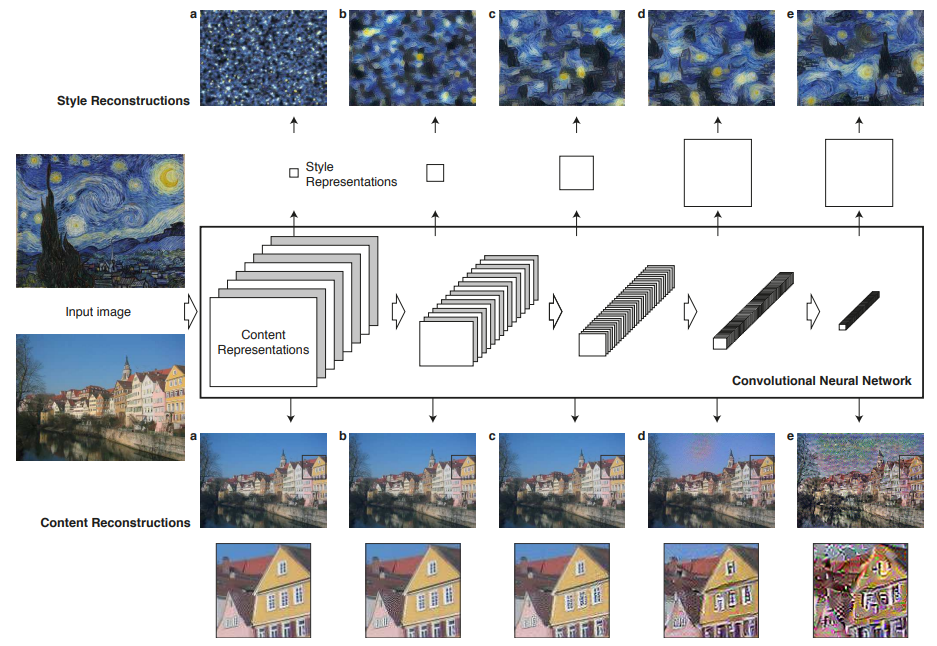
\includegraphics[width=\linewidth]{images/04_style.PNG}
여기서 살펴보면 input으로 하나는 target style이고 하나는 content 정보를 담당하는 image 두개가 들어온다. 목표는 style input에서 style 정보와 
content input에서 content 정보를 결합하여 새로운 이미지를 만들어내는 것이다. 위의 그림을 보면 layer가 깊어질 수록 style 정보(위에)가 더 뚜렷히 나타나며 content 정보은 거의 남아 있지 않다.
반면에 content 정보(아래)의 경우에는 layer가 깊어질수록 오히려 이미지 왜곡이 심해지는 것을 확인할 수 있다. 이는 layer가 깊어질수록 edge 정보를 잃기 때문이고 낮은 layer에서 오히려 edge 정보를
더 보존한다. 실험 구조는 아래와 같다. 
\newline  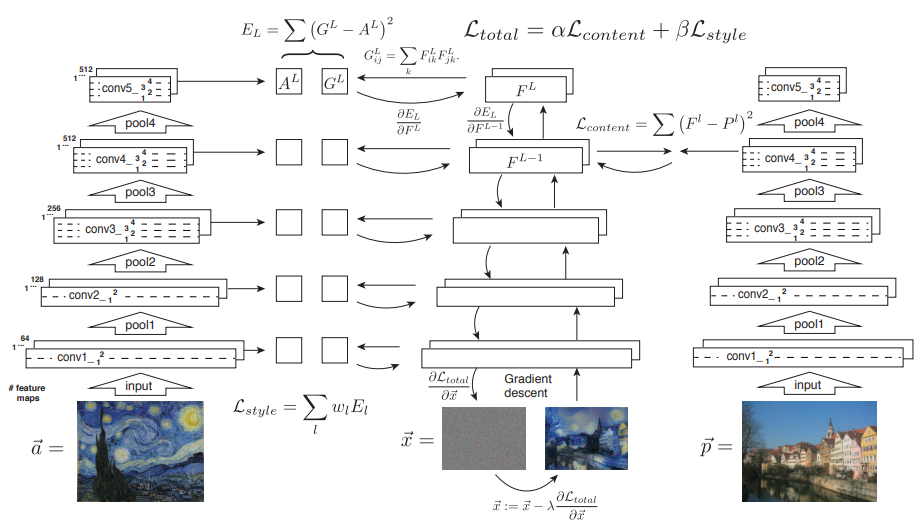
\includegraphics[width=\linewidth]{images/05_style.PNG}
style 정보는 각 layer별로 누적해서 구하고 content 정보는 conv4에서 얻은 feature로 비교하여 content 정보의 손실을 줄인다.

\subsection{Experiments}
\quad 그 결과 아래와 같이 content 정보는 보존되고 style이 변경되는 이미지를 얻을 수 있다.
\newline  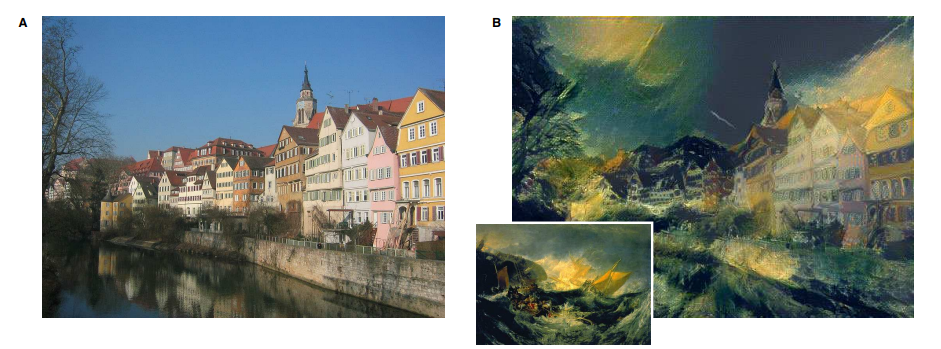
\includegraphics[width=6cm]{images/06_style.PNG}
\newline content정보와 style 정보 간에는 trade-off가 있다. 당연하게도 Loss function을 style loss와 content loss의 합으로 정의하였고 각기 다른 이미지에 
그 값을 받아오기 때문에 둘다 0으로 수렴하도록 움직이는 것이 불가능하다. 합이 최소로 되도록 update 될 뿐이다. 또한 CNN의 다른 layer에서 이미지를 뽑았을 때 결과가 차이가 있다.
마지막으로 style transfer의 특징으로 output이 무수히 많을 수 있기 때문에 input noise 초기화에 따라서 이미지가 차이가 난다.

\subsection{Conclusion}
\quad 이 논문에서는 CNN을 처음으로 이용하여서 Style transfer network을 설계했다는 것이 의의가 있다. 한계로는 style 정보를 정확하게 정의하는 것이 Gram matrix는 아닐 수 있다.
또한 forward backward를 같이 하며 noise 이미지로부터 새로운 이미지를 만드는 것이기 때문에 긴 시간이 소모된다는 단점이 있다.

\section{Perceptual Losses for real-time style transfer and super resolution \cite{johnson2016perceptual}}
 \subsection{motivation\cite{youtube}}
 \quad 앞선 논문의 단점은 forward와 backward가 함께 일어나며 실행시간이 오래 걸린다는 것이었다. 여기서는 어떻게 하면 실시간으로 적용가능한 style transfer을 설계할 수 있을지에 대한 고민에서 시작되었다.
 속도를 개선하고자 이 후 나온 style transfer의 경우에는 feed-forward network 방식을 채택하였다. 여기서는 feed-forward convolutional neural network using a per-pixel loss 와 보다 high-level feature을 비교하기 위해 perceptual loss를 결합하여 system을 만들었다. 
 그 결과 optimization based method와 비교해서 결과의 quality는 비슷하지만 3000배 가량 더 빠르다. 또한 super resolution에도 적용하였는데 per-pixel loss를 사용한 것보다 시각적으로 더 만족스러운 결과를 얻을 수 있었다.

 \subsection{Related Work}
 \quad feed-forward image transformation의 경우에는 기존 연구는 pixel 당 classification loss를 계산하여 model을 업데이트하였다. 
 이를 pixel 별이 아닌 CNN에서 추출한 high-level feature로 학습한 연구가 perceptual optimization이다.  
 
 \subsection{Method}
 \quad 이 논문에서 가장 중요한 것은 loss function의 선언이다. 그 전에 loss function을 구하기 위한 값을 추출하는 전체적인 구조는 아래와 같다.
 \newline  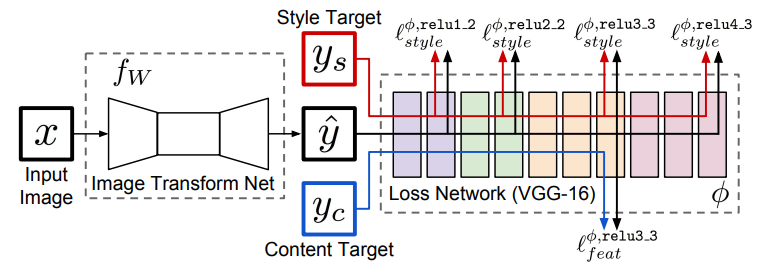
\includegraphics[width=\linewidth]{images/00_style.PNG}
  system은 크게 image transformation network $f_W$와 a loss network $\phi$로 나뉘어 진다. 먼저 image transformation network의 경우에는
  deep residual CNN을 사용한다. 이 때 나오는 output이 $\hat{y}$이다. loss는 output image $\hat{y}$ 과 target image $y_i$의 차이를 측정한 
  $l_i(\hat{y},y_i)$ 을 구할 것이다. loss network 부분은 학습 중에서는 freeze시킨 후 image transformation network을 학습시키는데 그 과정이 아래의 weight를 구하는 것이다.
  $$W^* = \underset{W}{argmin}E_{x,\{y_i\}}[\sum_{i=1}\lambda_il_i(f_W(x),y_i)]$$
  위의 식의 의미를 잠시 살펴보자면 loss network에 통과된 부분의 loss 값을 $\lambda$로 페널티를 줘서 더하는 형태로 이루어지고 이 합이 최소가 되도록 network를 학습시키게 된다.
  이 loss function은 두가지 종류가 있다. feature reconstruction loss $l_{feat}^{\phi}$ 과 style reconstruction loss $l_{style}^{\phi}$ 로 나뉘는데 각각은 content target $y_c$와 style target $y_s$와 계산을 하게 된다.
  임의의 input image로 style transfer를 적용시키기 위해 content target $y_c$와 style target $y_s$를 적절히 결합하여야 한다. 이 논문에서 image transform Net의 경우 5개의 
  residual block으로 이루어져 있고 batch normalization과 ReLU 사용하였다. 처음과 마지막 layer의 kernel 크기만 9x9 이고 그 외의 모든 convolutional layers은 3x3 kernel을 이용하였다.
  이 network를 통과하는 input의 값은 task에 따라 조금 다른데 style transfer의 경우에는 3x256x256이고 super-resolution task의 경우에는 upsampling factor f에 따라서 input을 3x256/fx256/f로 설정하였다.
  둘 다 나오는 output의 결과는 3x256x256으로 동일 하다. 또한 위의 구조 그림을 보면 알 수 있듯이 downsampling 후 upsampling을 하는 방법으로 network를 구성했는데 그 이유는 downsampling을 함으로써 계산상의 이점이 있고 보다 효율적으로 receptive field size를 늘릴 수 있기 때문이다. 
  perceptual loss function에 대해서 살펴보자. 먼저 볼 것은 feature reconstruction loss이다. 이 loss의 경우에는 $\hat{y}=f_W(x)$의 pixel 값을 target image y에 일치시키는 것 대신에 
  loss network를 추가적으로 통과시켜 보다 물체의 형태 같은 high-feature 정보을 학습시키는 것이다. 그 식은 아래와 같다.  
  $$l_{feat}^{\phi,j}(\hat{y},y) = \frac{1}{C_jH_jW_j}||\phi_j(\hat{y})-\phi_j(y))||^2$$
  이렇게 얻은 결과를 살펴보면 높은 layer로 갈수록 content 정보나 전체적인 spatial structure을 보존할지는 몰라도 정확한 shape 정보는 잃게된다. 
  \newline  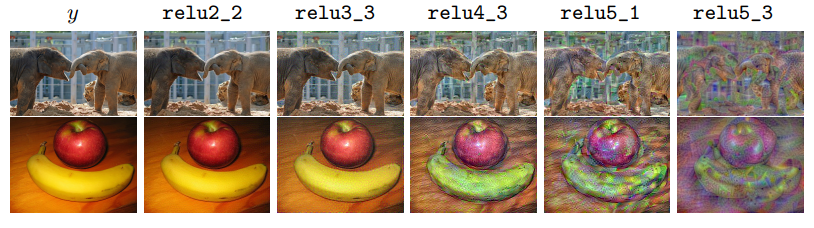
\includegraphics[width=\linewidth]{images/01_style.PNG}
  다음은 style reconstruction loss이다. 앞서 소개한 논문의 저자가 만든 channel간의 correlation을 구하는 Gram matrix를 이용한다. 
  $$G_j^{\phi}(x)_{c,c'} = \frac{1}{C_jH_jW_j}\sum_{h=1}^{H_j}\sum_{w=1}^{W_j}\phi_j(x)_{h,w,c}\phi_j(x)_{h,w,c'}$$
  여기서 $\phi_j(x)$는 jth layer에서의 activation이다. 이렇게 구한 Gram matrix로 아래와 같은 식을 이용해서 style reconstruction loss를 계산한다. 
  $$l_{style}^{\phi,j}(\hat{y},y) = ||G_j^{\phi}(\hat{y})-G_j^{\phi}(y)||^2$$ 
  이 때는 channel 갯수에 관계있는 Gram matrix이기 때문에 $\hat{y}$와 y의 size가 달라도 잘 정의 된다.
  \newline  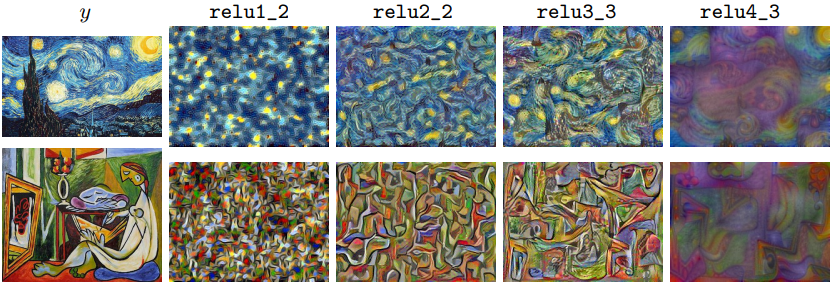
\includegraphics[width=\linewidth]{images/02_style.PNG}
  위의 그림을 보면 알 수 있다시피 style reconsturction loss는 stylistic feature을 잘 추출하는 반면 spatial structure은 무시된다.
  
  \subsection{Experiments}
  \quad  아래의 그림을 보면 object 정보를 보전하는 반면 배경 정보는 잃는 것을 확인 할 수 있다. 이로 보아 한 pixel별로 계산한것이 아니라 object의 feature 별로 loss를 계산했다는 것을 확인할 수 있다.
  \newline  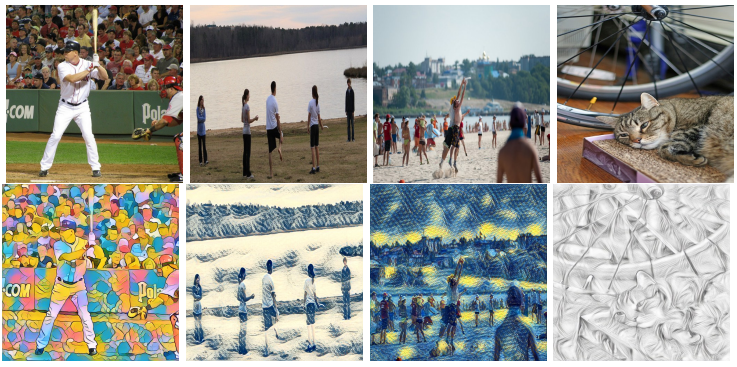
\includegraphics[width=6cm]{images/03_style.PNG}


  \subsection{Conclusion}
  \quad 이 논문에서는 feed-forward image transformation task의 빠름과 perceptual loss function의 high-level feature로 학습하는 system을 만든 결과 기존의 style transfer과 비슷하게 좋은 결과를 얻었고
  속도는 더 빨랐다. super resolution에 적용한 결과 SRCNN과 비교했을 때역시 pixel 별로 값이 차이가 나서 PSNR과 SSIM의 값은 더 낮게 나왔지만 그래도 edge 같은 부분을 더 선명하게 복원가능하였다. 다시말해 시각적으로 더 좋은 결과를 얻을 수 있었다.

\newpage
\bibliography{egbib}

\end{document}